
\chapter{Vue d'ensemble du système}\label{ch:systeme}

Le système est composé de plusieurs acteurs différents qui ont chacun une tâche bien précise. Ce chapitre propose une vue d'ensemble de ses éléments et explique également les interactions qui existent entre eux.

L'objectif du système est de permettre la récupération de toutes les données récoltées par le ou les capteurs et de centraliser ces informations afin que l'application mobile puisse les exploiter et les afficher aux utilisateurs au travers de son interface graphique.

Afin de pouvoir réaliser cet objectif, les éléments suivants sont développés.

\begin{itemize}
\item Un capteur
\item Une passerelle
\item Une base de données
\item Une application mobile
\end{itemize}

Le capteur est porté par un sportif, il est en charge de l'acquisition des données et de leur transmissions à une passerelle en utilisant la couche radio LoRa. Il est défini en détail dans le chapitre~\ref{ch:capteur}.

La passerelle se charge de récupérer les données transmises par le ou les capteurs, les traite et puis les centralise dans une base de données. Elle est décrite dans le chapitre~\ref{ch:passerelle}.

La base de données permet le stockage de toutes les informations collectées durant la course mais également d'autres informations qui sont saisies avant, comme le nom et prénom, le numéro de dossard ou le pays d'origine des athlètes. Chaque compétition ainsi que leurs informations associées sont également enregistrées dedans. Le chapitre~\ref{ch:bd} explique son fonctionnement.

L'application mobile est la fenêtre sur le système, elle permet aux utilisateurs de visualiser en temps réel l'évolution de la course. Sa description se trouve dans le chapitre~\ref{ch:app_mobile}.

Afin de pouvoir être utilisable pendant des compétitions sportives, le système doit être capable de gérer plusieurs capteurs en parallèle, il est donc développé dans cette optique. Cependant dans la mesure où dans le cadre du travail de Bachelor le projet est une preuve de concept, un seul capteur sera assemblé et testé. 

En ce qui concerne les passerelles, idéalement plusieurs d'entre elles doivent pouvoir être utilisées durant une course, cela permet de diminuer les zones d'ombres le long du parcours et également de minimiser le nombre de paquets perdus. Cependant cela complique passablement le système, car cela implique que la base de données doit être hébergée sur un serveur connecté à internet et donc que la passerelle doit également pouvoir s'y connecter. Afin de simplifier le développement du projet, il est décidé de ne développer qu'une seule passerelle et d'y héberger localement la base de données.

Enfin le chapitre~\ref{ch:produit} rassemble les éléments qu'il faudrait retravailler afin de faire de la preuve de concept un produit à part entière.

\section{Les interactions}

Le système exploite deux types de communication différentes afin de stocker et d'extraire des données de la base. D'une part la couche radio LoRa est utilisée pour la communication entre les capteurs et les passerelles, et d'autre part le WiFi pour les requêtes entre la base de données et l'application mobile. 

Dans le cadre de la preuve de concept et pour des raisons de simplification, la couche MAC LoRaWAN n'est pas employée, elle prendrait cependant tout son sens dans une optique de développement d'un produit.

La figure~\ref{fig:system_schema} montre les interactions existantes entre les acteurs du système.

\begin{figure}[htb]
\centering 
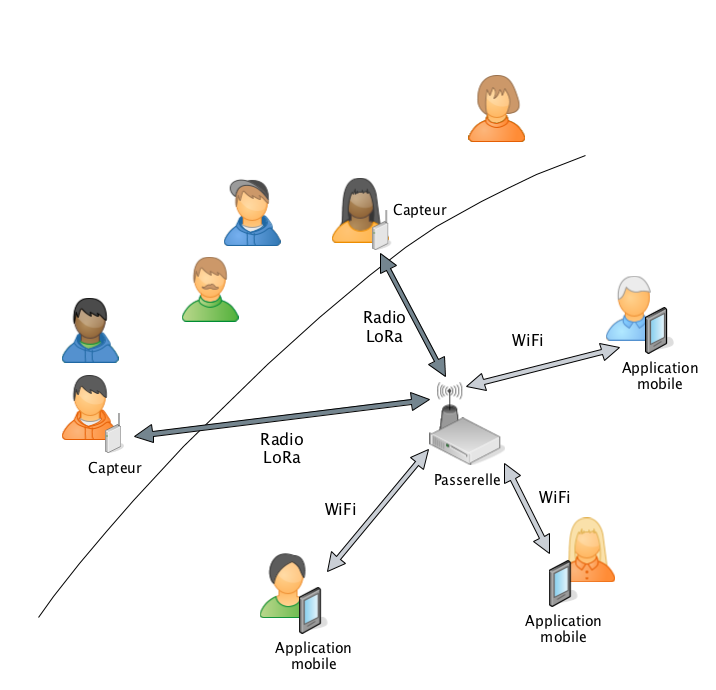
\includegraphics[width=0.9\columnwidth]{system_schema.png} 
\caption{Interactions des acteurs du système}
\label{fig:system_schema}
\end{figure}

\todo{Data flow?}

\section{LoRa \& LoRaWAN}\label{ch:lora_lorawan}

Lorsque l'on parle de LoRa, souvent une confusion est faite entre deux entités, d'un côté la couche LoRa et de l'autre la couche MAC LoRaWAN.

La couche physique LoRa est une technique de modulation pour les communications sans fil permettant l'envoi de données à bas débit à des distances de plusieurs kilomètres et le tout en consommant peu d'énergie. Ses caractéristiques rendent cette technologie très attractive pour des projets dans le monde de l'embarqué où les systèmes disposent de très peu de ressources et fonctionnent souvent avec des accumulateurs comme seule source d'énergie.

A son fondement, la couche physique est basée sur un type de modulation appelé modulation à étalement de spectre. Son principe premier est d'élargir artificiellement la bande de fréquence utilisée par le signal à envoyer, ce qui le rend du coup plus résilient aux interférences volontaires ou involontaires.

Une des techniques très connues dans ce type de modulation est l’étalement de spectre à séquence directe (Direct Sequence Spread Spectrum). Comme expliqué, du fait de l'utilisation de l'étalement de spectre ce signal est plus robuste aux interférences, par contre il nécessite que le transmetteur et le récepteur se mettent d’accord sur la séquence à utiliser pour encoder les signaux. Cette technique est beaucoup utilisée, notamment par la norme 802.11b (WiFi). Elle comporte comme gros désavantage le fait qu’elle nécessite une horloge de base très précise et que le décodage du signal sur le récepteur peut être long en fonction de la séquence de codage utilisée. Tout ceci rend cette technique peu pratique pour des systèmes à bas coût et à basse consommation comme ceux du domaine de l’Internet of Things (IoT).

Dans les années 40, une autre technique se basant sur l’étalement de spectre a été développée pour être utilisée dans les applications radars, le Chirp Spread Spectrum (CSS). Elle utilise toujours le principe d’étalement de spectre afin d’être robuste aux interférences, cependant l’utilisation d’une séquence pseudo aléatoire qui est utilisée pour distinguer le signal du bruit, comme dans les techniques Direct Sequence Spread Spectrum (DSSS) ou Frequency Hopping Spread Spectrum (FHSS), ne se fait plus. En plus des avantages inhérents à l’étalement de spectre, les changements liés à cette technique la rendent résistante à la dégradation des données causées par les trajets multiples (multipath) et l’évanouissement (fading). \cite{lora_modulation_basics}

Un autre élément intéressant est apporté par la couche physique LoRa, le facteur d'étalement du spectre. Ce paramètre configurable définit comme son nom l'indique le facteur d'étalement du spectre lors de la modulation du signal. Plus le facteur est grand, plus la transmission de l’information sera lente mais par contre la portée de réception des données sera grande. Plus le facteur est petit et plus le taux de transfert sera important, par contre la portée en sera grandement réduite. Ce facteur peut prendre une valeur entre 7 et 12, ce qui permet de faire un choix entre une distance accrue ou un taux de transfert plus élevé, entre 0.3 kbps avec un facteur de 12 et 27 kbps pour l'autre extrême. Enfin, ce paramètre influence également sur la taille de la charge utile qu'il est possible d'envoyer dans un seul message, entre 51 octets pour la valeur la plus faible et 222 octets maximum. \cite{limits_lorawan}

La modulation LoRa utilise les bande de fréquences ISM (industrielle, scientifique, médicale), qui sont libres d'utilisation et sans surcoût, à condition de respecter les duty cycle assignés. En effet, puisque cette bande de fréquence n'est pas contrôlée, des quota de taux d'utilisation ont été définis afin de garantir que tous les utilisateurs puissent envoyer leurs données et ainsi éviter qu'un petit nombre de capteur ne monopolise la bande de fréquence. \cite{ism_bands}

La table \ref{tab:bande_ism} présente les quota pour quelques bandes de fréquence.

\begin{table}[htb]
\caption{Quota d'utilisation de la bande ISM}
\label{tab:bande_ism}
\centering
\begin{tabular}{ l l l }
\toprule
Code & Fréquence [Mhz] & Duty cycle \\
\midrule
g & 863.0 à 868.0 & 1\% \\
g1 & 868.0 à 868.6 & 1\% \\
g2 & 868.7 à 869.2 & 0.1\% \\
g3 & 869.4 à 869.65 & 10\% \\
\bottomrule 
\end{tabular}
\end{table}

LoRaWAN, qui est souvent également appelé à tord LoRA, est la couche MAC qui s'appuie directement sur la couche radio. Elle propose un set de fonctionnalités supplémentaires permettant de faciliter la gestion d'un grand nombre de capteurs et d'améliorer le niveau de sécurité. Son concept est de s'appuyer sur un réseau de passerelles placées afin de produire une couverture maximale pour les utilisateurs. Les passerelles récupèrent les paquets et les transmettent à un serveur central, le serveur réseau, qui gère le protocole dans son ensemble. Il s'occupe de générer les paquets de réponses qui sont envoyés en retour aux passerelles et il permet également l'envoi des données reçues des capteurs à des serveurs d'applications qui vont ensuite exploiter les données. LoRaWAN permet l'encryption des données transitant entre le serveur réseau et les capteurs, qui sont les deux seuls éléments à connaître les clefs de chiffrement, ce qui permet d'assurer la confidentialité des informations traversant le réseau. Une autre fonctionnalité intéressante que ce protocole propose est le Adaptive Data Rate (ADR), en fonction des paramètres reçus des passerelles et des informations concernant la qualité de transmission des capteurs, le serveur réseau va pouvoir altérer les débits de transfert des capteurs. Un nœud qui sera très distant de la passerelle verra son taux de transfert baissé, ce qui permettra de rendre la communication plus robuste aux interférences. \cite{lorawan_spec}

Pour des raisons de simplification, le projet du travail de Bachelor utilise uniquement la couche radio LoRa sans la couche protocolaire LoRaWAN. En effet, la couche LoRaWAN est très intéressante dans le cas d'utilisation d'un produit où plusieurs capteurs devraient être gérés en parallèle. Dans ce cas, il est obligatoire de stocker les données sur internet et LoRaWAN propose toute une infrastructure permettant de le faire, en plus cela permet d'utiliser des technologies web modernes pour accéder aux données, des API REST par exemple. Cependant, puisque ce projet a pour objectif de valider les études que j'ai effectuées dans la filière informatique embarquée, j'ai préféré me concentrer sur le développement dans ce domaine et donner une priorité plus basse aux éléments qui en sortiraient.

\begin{figure}[htb]
\centering 
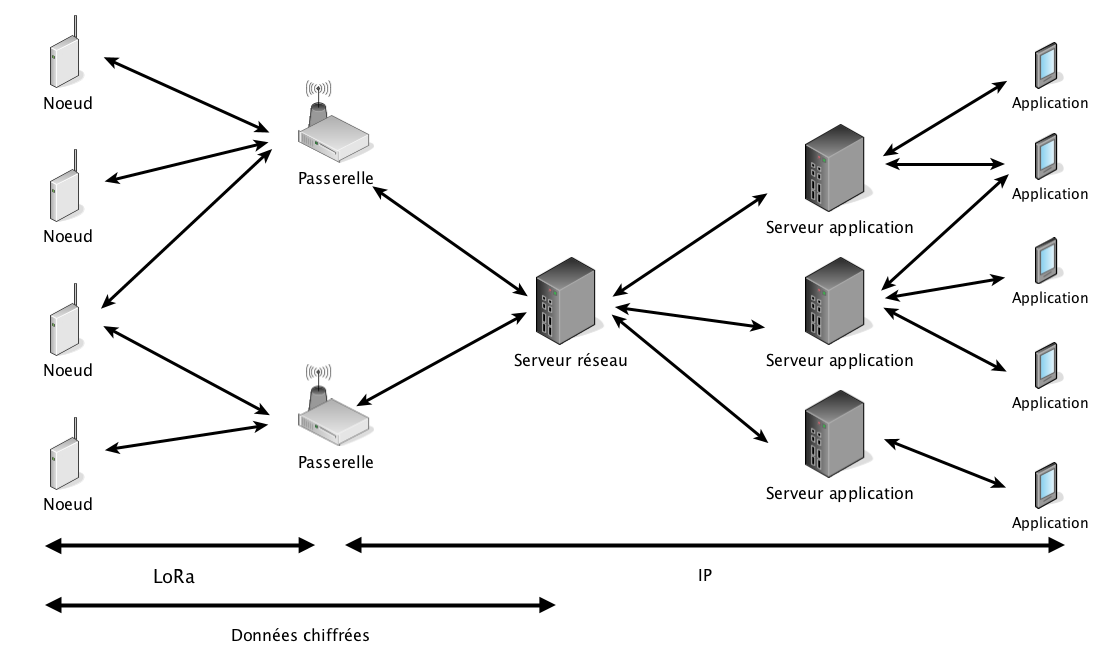
\includegraphics[width=1\columnwidth]{lorawan_infra.png} 
\caption{Infrastructure LoRaWAN}
\label{fig:infra_lorawan}
\end{figure}